\chapter[Homological Prereqs]{Manifolds, Simplexes Complexes, and Triangulability: Building Blocks}

\section{Manifolds}
We define some basic Euclidean sets for use in homeomorphisms.
\begin{definition}
  The \emph{$n$-dimensional cube}, denoted $\DD^n$, is defined as
  \begin{align*}
    \DD^n
    &= \set{\pn{x_1, \ldots, x_n} \in \RR^n \MID 0 \leq x_i \leq 1 \text{ for } i = 1, \ldots, n} \\
    &= \overbrace{[0,1] \times [0,1] \times \cdots \times [0,1]}_{n \text{ times}} \subset \RR^n.
  \end{align*}
\end{definition}
\begin{definition}
  The \emph{standard $n$-ball}, denoted $B^n$, is
  \[
    B^n = \set{\pn{x_1, \ldots, x_n} \in \RR^n \MID x_1^2 + \cdots + x^2_n \leq
      1}.
  \]
\end{definition}
\begin{definition}
  The \emph{standard $n$-sphere}, denoted $\Ss^n$, is
  \[
    \Ss^n = \set{(x_0, \ldots, x_n) \in \RR^{n+1} \MID x^2_0 + \cdots + x^2_n =
      1}.
  \]
  note that here, our indices start at $0$.
\end{definition}
\begin{definition}
  An \emph{$n$-dimensional manifold} or \emph{$n$-manifold} is a separable
  metric space $M$ such that $\forall p \in M$, $\exists U \in \ms T(M) \st p
  \in U$ and $U \cong V \subset \RR^n$.
\end{definition}
\begin{problem}[15.8]
  If $M$ is an $n$-manifold and $U$ is an open subset of $M$, then $U$ is also
  an $n$-manifold.
\end{problem}
\begin{problem}[15.9]
  If $M$ is an $m$-manifold and $N$ is an $n$-manifold, then $M \times N$ is an
  $(m+n)$-manifold.
\end{problem}
\begin{problem}[15.10]
  Let $M^n$ be an $n$-dimensional manifold with boundary. Then $\partial M^n$ is
  an $(n-1)$-manifold.
\end{problem}
\section{Simplicial Complexes}~
\begin{definition}[Affine Independence]
  Let $X = \set{v_0, \ldots, v_k} \subset \RR^n$. We say $X$ is \emph{affinely
    independent} if $\set{v_1 - v_i, \ldots, v_k - v_i}$ is linearly
  independent for all $v_i$.
\end{definition}
\begin{example}
  $X = \set{(0,1), (-\sqrt{3}/2, -1/2), (\sqrt{3}/2, -1/2)}$ is affinely
  independent.
\end{example}
\begin{definition}[Convex combination]
  A \emph{convex combination} of $v_0, \ldots, v_k$ is a linear combination
  of these points whose coefficients are nonnegative and sum to 1.
\end{definition}
\begin{definition}
  A \emph{$k$-simplex} is the set of all convex combinations of $k+1$ affinely
  independent points in $\RR^n$. For affinely independent points $v_0, \ldots,
  v_k$ in $\RR^n$, $\set{v_0\cdots v_k}$ denotes the $k$-simplex
  \[
    \set{\lambda_0 v_0 + \lambda_1v_1 + \cdots + \lambda_kv_k \MID \forall i -
      1, \ldots, k;\ 0 \leq \lambda_i \leq 1 \text{ and } \sum_{i=0}^k \lambda_i
    = 1}
  \]
  each $v_i$ is called a \emph{vertex} of $\set{v_0 \cdots v_k}$. Any point $x$
  in the $k$-simplex is specified uniquely by the $k+1$ coefficients
  $(\lambda_i)$; these coefficients are called the \emph{barycentric coordinates
    of $x$.} The \emph{barycentric coordinate of $x$ with respect to vertex
    $v_i$} is the coefficient $\lambda_i$.
\end{definition}
\begin{definition}
  Any simplex $\tau$ whose vertices are a nonempty subset of the vertices of a
  $k$-simplex $\sigma$ is called a \emph{face} of $\sigma$. If the number of
  vertices is $i+1$, then $\tau$ has \emph{dimension} $i$ and is called an
  $i$-face of $\sigma$ and $\tau$ has \emph{codimension} $k-i$, the number of
  dimensions below the top dimension.
\end{definition}
\textbf{Notational Note:} if $\sigma = \simp k$, the $(k-1)$-dimensional face of
$\sigma$ obtained by deleting the vertex $v_j$ from the list of vertices of
$\sigma$ is denoted by $\simpdel{i}{k}$.
\begin{problem}[15.11]
  Show that if $\sigma$ is a simplex and $\tau$ is one of its faces, then $\tau
  \subset \sigma$.
\end{problem}
\begin{solution}
  This is fairly trivial, so we offer just a sketch. Suppose $\mb v \in \tau$.
  Then write $\mb v$ as an element of $\sigma$ by taking $\lambda_i = 0$ for all
  those $v_i \not \in \tau$.
\end{solution}
\begin{definition}
  A \emph{simplicial complex} $K$ (in $\RR^n$) is a collection of simplicies in
  $\RR^n$ satisfying the following conditions.
  \begin{enumerate}[label=\arabic*.]
    \item If a simplex $\sigma$ is in $K$, then each face of $\sigma$ is also in
      $K$.
    \item Any two simplices in $K$ are either disjoint or their intersection is
      a face of each.
  \end{enumerate}
\end{definition}
\begin{problem}[15.13]
  Exhibit a collection of simplices that satisfies condition (1) but not
  condition (2) in the definition of a simplicial complex.
\end{problem}
\begin{solution}
  Consider the following diagram, where the interior of each simplex is taken to
  be in the complex.
  \begin{figure}[H]
    \centering
    \begin{tikzpicture}[every node/.style={circle,draw=black, fill=white, inner sep=0pt,minimum size=7pt}]
      % Simplex 1
      \coordinate (A) at (0,0);
      \coordinate (B) at (3,4.5);
      \coordinate (C) at (5,-1);

      % Simplex 2
      \coordinate (D) at (2.5,1);
      \coordinate (E) at (6,3.8);
      \coordinate (F) at (9,.5);

      \draw[fill=blue!50!white, fill opacity=.5] (A) -- (B) -- (C) -- (A);
      \draw[fill=red!50!white, fill opacity=.5] (D) -- (E) -- (F) -- (D);

      \draw[name path=B--C] (B) -- (C);
      \draw[name path=D--E] (D) -- (E);
      \draw[name path=D--F] (D) -- (F);

      \path[name intersections={of=B--C and D--E, by=G}];
      \path[name intersections={of=B--C and D--F, by=H}];

      % nodes for simplex (1)
      \node (a) at (A) {};
      \node (b) at (B) {};
      \node (c) at (C) {};

      % nodes for simplex (2)
      \node (d) at (D) {};
      \node (e) at (E) {};
      \node (f) at (F) {};
    \end{tikzpicture}
    \caption{An unfortunate collision}
    \label{fig:non-simplicial-complex}
  \end{figure}
  Note that to fix this sorry situation, we can't just add two vertices at the
  points of intersections of the lines above (then the intersection of the
  resulting simplex with the two shone above would be non-trivial, but still not
  a face of the larger ones). We'd actually need something much more
  complicated.
  \begin{figure}[H]
    \centering
    \begin{tikzpicture}[every node/.style={circle,draw=black, fill=white, inner sep=0pt,minimum size=7pt}]
      % Simplex 1
      \coordinate (A) at (0,0);
      \coordinate (B) at (3,4.5);
      \coordinate (C) at (5,-1);

      % Simplex 2
      \coordinate (D) at (2.5,1);
      \coordinate (E) at (6,3.8);
      \coordinate (F) at (9,.5);

      \draw[fill=blue!50!white, fill opacity=.5] (A) -- (B) -- (C) -- (A);
      \draw[fill=red!50!white, fill opacity=.5] (D) -- (E) -- (F) -- (D);

      \draw[name path=B--C] (B) -- (C);
      \draw[name path=D--E] (D) -- (E);
      \draw[name path=D--F] (D) -- (F);

      \path[name intersections={of=B--C and D--E, by=G}];
      \path[name intersections={of=B--C and D--F, by=H}];

      \draw[dashed] (B) -- (E);
      \draw[dashed] (C) -- (F);
      \draw[dashed] (A) -- (D);
      \draw[dashed] (D) -- (B);
      \draw[dashed] (D) -- (C);

      \node (g) at (G) {};
      \node (h) at (H) {};

      % nodes for simplex (1)
      \node (a) at (A) {};
      \node (b) at (B) {};
      \node (c) at (C) {};

      % nodes for simplex (2)
      \node (d) at (D) {};
      \node (e) at (E) {};
      \node (f) at (F) {};
    \end{tikzpicture}
    \caption{Constructing a resolution}
    \label{fig:non-simplicial-complex}
  \end{figure}
  \begin{figure}[H]
    \centering
    \begin{tikzpicture}[every node/.style={circle,draw=black, fill=white, inner sep=0pt,minimum size=7pt}]
      % Simplex 1
      \coordinate (A) at (0,0);
      \coordinate (B) at (3,4.5);
      \coordinate (C) at (5,-1);

      % Simplex 2
      \coordinate (D) at (2.5,1);
      \coordinate (E) at (6,3.8);
      \coordinate (F) at (9,.5);

      \draw[fill=blue!50!white, fill opacity=.5] (A) -- (B) -- (C) -- (A);
      \draw[fill=red!50!white, fill opacity=.5] (D) -- (E) -- (F) -- (D);

      \draw[name path=B--C] (B) -- (C);
      \draw[name path=D--E] (D) -- (E);
      \draw[name path=D--F] (D) -- (F);

      \path[name intersections={of=B--C and D--E, by=G}];
      \path[name intersections={of=B--C and D--F, by=H}];

      \draw[fill=green!30!white] (B) -- (G) -- (D) -- (B);
      \draw[fill=orange!30!white] (H) -- (C) -- (D) -- (H);
      \draw[fill=pink!30!white] (A) -- (B) -- (D) -- (A);
      \draw[fill=teal!25!white] (B) -- (E) -- (G) -- (B);
      \draw[fill=black!10!white] (H) -- (F) -- (C) -- (H);

      \node (g) at (G) {};
      \node (h) at (H) {};

      % nodes for simplex (1)
      \node (a) at (A) {};
      \node (b) at (B) {};
      \node (c) at (C) {};

      % nodes for simplex (2)
      \node (d) at (D) {};
      \node (e) at (E) {};
      \node (f) at (F) {};
    \end{tikzpicture}
    \caption{The completed resolution}
    \label{fig:non-simplicial-complex}
  \end{figure}
\end{solution}
\begin{definition}
  The \emph{underlying space} $\abs{K}$ of a simplicial complex $K$ is the set
  \[
    \abs{K} = \bigcup_{\sigma \in K} \sigma,
  \]
  the union of all simplices in $K$, with a topology consisting of sets whose
  intersection with each simplex $\sigma \in K$ is open in $\sigma$. For finite
  simplicial complexes, this topology is the topology inherited as a subspace of
  $\RR^n$.
\end{definition}
\begin{problem}[15.14]
  Let $K$ be the following simplicial complex:
  \[
    \text{(Omitted because it takes a long time to TeX out)}
  \]
  draw $K$ and its underlying space.
\end{problem}
\begin{solution}
  \begin{figure}[H]
    \centering
    \begin{minipage}{.49\linewidth}
      \centering
      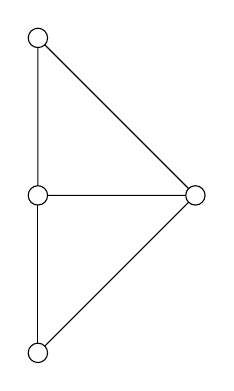
\begin{tikzpicture}[scale=2, every node/.style={circle,draw=black, fill=white, inner sep=0pt,minimum size=7pt}]

        \coordinate (A) at (0,0);
        \coordinate (B) at (0,1);
        \coordinate (C) at (1,0);
        \coordinate (D) at (0,-1);

        \draw (A) -- (B) -- (C) -- (A);
        \draw (A) -- (D);
        \draw (D) -- (C);

        \node (a) at (A) {};
        \node (b) at (B) {};
        \node (c) at (C) {};
        \node (d) at (D) {};

      \end{tikzpicture}
    \end{minipage}
    \begin{minipage}{.49\linewidth}
      \centering
      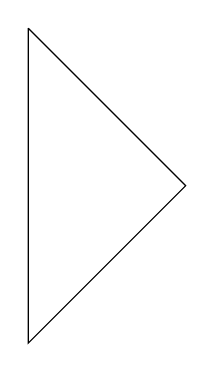
\begin{tikzpicture}[scale=2, every node/.style={circle,draw=black, fill=white, inner sep=0pt,minimum size=7pt}]

        \coordinate (B) at (0,1);
        \coordinate (C) at (1,0);
        \coordinate (D) at (0,-1);

        \draw (B) -- (C) -- (D) -- (B);
      \end{tikzpicture}
    \end{minipage}
    \caption{$K$ (left) and its underlying space (right).}
  \end{figure}
\end{solution}
\begin{definition}
  A topological space $X$ is said to be \emph{triangulable} if it is
  homeomorphic to the underlying space of a simplicial complex $K$. In that
  case, we say $K$ is a \emph{triangulation} of $X$.
\end{definition}
\begin{problem}[15.15]
  Show that the space shown in Figure 15.2 (not included here) is triangulable
  by exhibiting a simplicial complex whose underlying space it is homeomorphic
  to.
\end{problem}
\begin{solution}
  \begin{figure}[H]
    \centering
    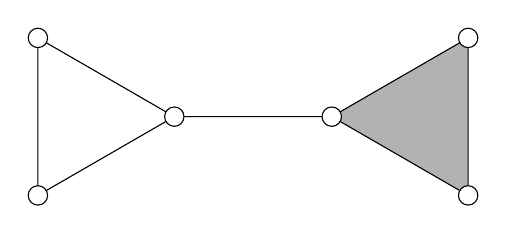
\begin{tikzpicture}[scale=2, every node/.style={circle,draw=black, fill=white, inner sep=0pt,minimum size=7pt}]

      \coordinate (A) at (0,0);
      \coordinate (B) at (-.866,.5);
      \coordinate (C) at (-.866,-.5);
      \coordinate (D) at (1,0);
      \coordinate (E) at (1.866,.5);
      \coordinate (F) at (1.866,-.5);

      \draw (A) -- (B) -- (C) -- (A) -- (D);
      \draw[fill=black!30!white] (D) -- (E) -- (F) -- (D);

      \node (a) at (A) {};
      \node (b) at (B) {};
      \node (c) at (C) {};
      \node (d) at (D) {};
      \node (e) at (E) {};
      \node (f) at (F) {};

    \end{tikzpicture}
    \caption{Such a simplicial complex. Note, the left triangle is unfilled.}
  \end{figure}
\end{solution}
\begin{problem}[15.6]
  For each $n \in \NN$, $\Ss^n$ is triangulable.
\end{problem}
\begin{proof}
  We proceed by induction.

  \begin{induction}
    \item Note that $S^0$ is trivially triangulable by taking $K =
      \set{\set{v_0}, \set{v_2}}$.
    \item Suppose that for $k \in \NN \cup \set{0}$, $\Ss^k$ is triangulable by
      a simplicial complex $K$.
    \item Take $v_{k+1} \in \RR^{k+1}$ such that $v_{k+1} \in
      (\vspan{K})^\perp$. Then
  \end{induction}
  {\color{red} This proof is unfinished. Hey, future Forest --- you should
    return to this later!}
\end{proof}
\section{Simplicial Maps and PL Homeomorphisms}
We now define structure-preserving maps bewteen simplicial concepts.
\begin{definition}
  Let $X,Y$ be topological spaces. A function $f : X \to Y$ is called a
  \emph{simplicial map} iff there exist simplicial complexes $K$ and $L$ such
  that $\abs{K} = X$, $\abs{L} = Y$, and $f$ maps each simplex of $K$ linearly
  onto a (possibly lower-dimensional) simplex in $L$.
\end{definition}
\begin{definition}
  A simplicial map $f$ is a simplicial homomorphism iff it's a bijection; in
  that case, the two complexes are \emph{simplicially homeomorphic}
\end{definition}
\begin{problem}[15.17]
  A simplicial map from $K$ to $L$ is determined by the images of the vertices
  of $K$.
\end{problem}
\begin{solution}
  Apply linearity and show the analog of images of liner combinations being
  uniquely determined by the action on the basis.
\end{solution}
\begin{problem}[15.18]
  A composition of simplicial maps is a simplicial map.
\end{problem}
\begin{solution}
  Simply plug in arbitrary points and verify the properties hold.
\end{solution}
\begin{definition}
  Let $K$ be a simplicial complex. Then a simplicial complex $K'$ is a
  \emph{subdivision} of $K$ iff each simplex of $K'$ is a subset of a simplex of
  $K$ and each simplex of $K$ is the union of finitely many simplices of $K'$.
\end{definition}
\begin{definition}
  If $K$ and $L$ are complexes, a continuous map $f : \abs{K} \to \abs{L}$ is
  called \emph{piecewise linear} or \emph{PL} if and only if there are
  subdivisions $K'$ of $K$ and $L'$ of $L$ such that $f$ is a simplicial map
  from $K'$ to $L'$. If there exist subdivisions such that $f$ is a simplicial
  homomorphism, then $f$ is a \emph{PL homomorphism} and the spaces are \emph{PL
  homeomorphic.}
\end{definition}
\begin{problem}[15.21]
  A composition of PL maps is PL. A PL homeomorphism is an equivalence relation.
\end{problem}
\begin{problem}[15.22]
  PL homeomorphic complexes are homeomorphic as topological spaces.
\end{problem}


%%% Local Variables:
%%% TeX-master: "main"
%%% End: